\section{Descripción del prototipo}
Esta interfaz de programación de aplicaciones provee acceso al sistema de archivos distribuído de \emph{Hadoop}, tanto para operaciones de lectura como de escritura. Esta herramienta permite la interacción del programador con la configuración y ejecución de los algoritmos de minería de datos implementados en \emph{Luminus}. Asímismo, permite a cualquier programador Java añadir sus propios algoritmos programados con el paradigma MapReduce.
\section{Análisis}
Inicialmente se tenía contemplado hacer uso de un sitio web para presentar los resultados de la ejecución de los algoritmos de minería de datos que contiene \emph{Luminus}. Sin embargo, durante fases posteriores del proyecto, se tomó la decisión de que sería de mayor utilidad presentarlos por medio de una interfaz de programación de aplicaciones (API). De esta forma \emph{Luminus} se vuelve una herramienta reutilizable y mucho más versátil.
\subsection{Casos de uso}
A continuación se muestran los casos de uso encontrados para este aplicativo 
\begin{figure}[H]
	\hypertarget{fig:confi}{\hspace{1pt}}
	\begin{center}	
		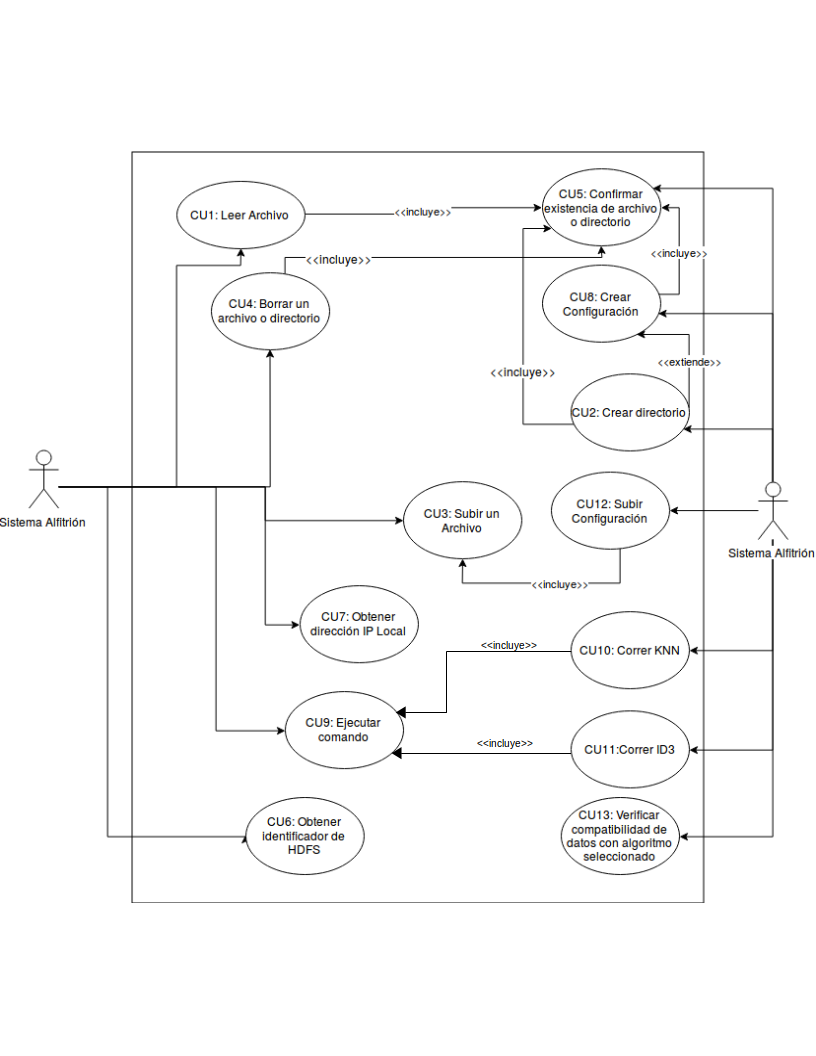
\includegraphics[width=1\textwidth]{capitulo4b/images/cu1.png}
		\caption{Diagrama de casos de uso}
		\label{fig:confi}
	\end{center}
\end{figure}
\begin{UseCase}{CU1}{Leer archivo}{
	Lee un archivo del sistema de archivos distribuidos a un stream especificado.
}

	\UCitem{Versión}{\color{Gray}1.0}

	\UCitem{Autor}{\color{Gray}Mayra Patricia Tovar Barba y Kevin Raúl Monteón Valdes.}

	\UCitem{Supervisa}{\color{Gray}Ulises Vélez Saldaña y Alejandro Botello Castillo.}

	\UCitem{Actor}{Usuario Experto, Sistema.}

	\UCitem{Propósito}{Obtener el contenido de un archivo del HDFS.}

	\UCitem{Entradas}{Ruta de archivo, Stream de salida, Identificador de HDFS, Dirección IP del Nodo Maestro.}

	\UCitem{Origen}{Código que implementa la API.}

	\UCitem{Salidas}{Ninguna.}

	\UCitem{Destino}{Stream de salida.}

	\UCitem{Precondiciones}{Debe existir el archivo de la ruta especificada.\newline El HDFS es accesible por la red.}

	\UCitem{Postcondiciones}{Los bytes del archivo habrán sido enviado a través del stream de salida.}

	\UCitem{Errores}{LuminusException(1) \refMSG{MSG1}{No existe el archivo o directorio}, IOException.}

	\UCitem{Tipo}{Caso de uso primario.}

	\UCitem{Observaciones}{}

\end{UseCase}

%--------------------------------------

\begin{UCtrayectoria}

	\UCpaso[\UCactor] Invoca el método getDataFromFile.

	\UCpaso[\UCactor] Envía [{\em Ruta del Archivo}].

	\UCpaso[\UCactor] Envía [{\em Stream de Salida}].

	\UCpaso[\UCactor] Envía [{\em Identificador de HDFS}].

	\UCpaso[\UCactor] Envía [{\em Dirección IP del Nodo Maestro}].

	\UCpaso[\UCsist] Realiza una conexión al nodo maestro del HDFS por medio de la [{\em Dirección IP del Nodo Maestro}].\label{CU1conexion}

	\UCpaso[\UCsist] Verifica que la [{\em Ruta del Archivo}] exista. \refTray{A}

	\UCpaso[\UCsist] Copia en el [{\em Stream de Salida}] la información contenida en el archivo. \refTray{B}

	\UCpaso[\UCsist] Cierra la conexión al nodo maestro del HDFS creada en el paso \ref{CU1conexion}.

	\UCpaso[] Termina el caso de uso.

\end{UCtrayectoria}


%--------------------------------------		

	\begin{UCtrayectoriaA}{A}{Archivo o directorio no encontrado}

		\UCpaso Manda el Mensaje \refMSG{MSG1}{No existe el archivo o directorio}.

		\UCpaso[] Termina el caso de uso.

	\end{UCtrayectoriaA}

	

%--------------------------------------

	\begin{UCtrayectoriaA}{B}{Error al copiar}

		\UCpaso Manda el Mensaje con la información proporcionada por Java acerca del error de escritura o lectura.

		\UCpaso[] Termina el caso de uso.

	\end{UCtrayectoriaA}



%%%%%%%%%%%%%%%%%%%%%%%%%%%%%%%%%%%%%%%%%%%%%%%%%%%%%%%%%%%%%%%%

\begin{UseCase}{CU2}{Crear directorio}{

Crea un directorio en el sistema de archivos distribuido de Hadoop (HDFS).

}

\UCitem{Versión}{\color{Gray}0.1}

\UCitem{Autor}{\color{Gray}Mayra Patricia Tovar Barba y Kevin Raúl Monteón Valdes}

\UCitem{Supervisa}{\color{Gray}Ulises Vélez Saldaña y Alejandro Botello Castillo}

\UCitem{Actor}{Usuario Experto, Sistema.}

\UCitem{Propósito}{Crear un directorio en el HDFS.}

\UCitem{Entradas}{Ruta de directorio, Identificador de HDFS, Dirección IP del Nodo Maestro.}

\UCitem{Origen}{Código fuente}

\UCitem{Salidas}{Nuevo directorio en el HDFS.}

\UCitem{Destino}{Ninguno.}

\UCitem{Precondiciones}{No debe existir el directorio en la [{\em Ruta del directorio}] especificada.\newline El HDFS es accesible por la red.}

\UCitem{Postcondiciones}{Se crea un nuevo directorio en la [{\em Ruta del directorio}] especificada.}

\UCitem{Errores}{LuminusException(3) \refMSG{MSG3}{El directorio ya existe}}

\UCitem{Tipo}{Caso de uso primario.}

\UCitem{Observaciones}{}

\end{UseCase}

%--------------------------------------

\begin{UCtrayectoria}

\UCpaso[\UCactor] Invoca al método makeHDFSDirectory

\UCpaso[\UCactor] Envía [{\em Ruta de directorio}].

\UCpaso[\UCactor] Envía [{\em Identificador de HDFS}].

\UCpaso[\UCactor] Envía [{\em Dirección IP del Nodo Maestro}].

\UCpaso[\UCsist] Realiza una conexión al nodo maestro del HDFS por medio del [{\em Identificador de HDFS}]\label{CU2conexion}

\UCpaso[\UCsist] Verifica que la [{\em Ruta del directorio}] no exista \refTray{A}

\UCpaso[\UCsist] Crea un nuevo directorio en la [{\em Ruta del directorio}] especificada.

\UCpaso[\UCsist] Cierra la conexión al nodo maestro del HDFS creada en el paso \ref{CU2conexion}

\UCpaso[] Termina el caso de uso.

\end{UCtrayectoria}



%--------------------------------------		

\begin{UCtrayectoriaA}{A}{Directorio ya existe}

	\UCpaso Manda el Mensaje \refMSG{MSG3}{El directorio ya existe}.

	\UCpaso[] Termina el caso de uso.

\end{UCtrayectoriaA}


\subsection{Puntos de extensión}
\UCExtensionPoint{
	% Cuando:
	El directorio que se desea crear corresponde a un directorio de configuración
}{
	% Durante la región:
	Del paso 7 al paso 9.
}{
	% Casos de uso a los que extiende:
}{
	\hyperlink{CU8}{CU8 Crear Configuración}.
}
%%%%%%%%%%%%%%%%%%%%%%%%%%%%%%%%%%%%%%%%%%%%%%%%%%%%%%%%%%%%%%%%

\begin{UseCase}{CU3}{Subir un archivo}{

Copia un archivo local al sistema de archivos distribuido de Hadoop (HDFS).

}

\UCitem{Versión}{\color{Gray}0.1}

\UCitem{Autor}{\color{Gray}Mayra Patricia Tovar Barba y Kevin Raúl Monteón Valdes}

\UCitem{Supervisa}{\color{Gray}Ulises Vélez Saldaña y Alejandro Botello Castillo.}

\UCitem{Actor}{Usuario Experto, Sistema.}

\UCitem{Propósito}{Sube un archivo al HDFS.}

\UCitem{Entradas}{Ruta de archivo local, Ruta de archivo remoto, Identificador de HDFS, Bandera de Sobrescribir.}

\UCitem{Origen}{Código fuente}

\UCitem{Salidas}{Nuevo archivo en el HDFS.}

\UCitem{Destino}{Ninguno.}

\UCitem{Precondiciones}{El HDFS es accesible por la red.}

\UCitem{Postcondiciones}{Se crea o actualiza un archivo en la [{\em Ruta de archivo remoto}] especificada.}

\UCitem{Errores}{LuminusException(3)\refMSG{MSG3}{El directorio ya existe}}

\UCitem{Tipo}{Caso de uso primario.}

\UCitem{Observaciones}{}

\end{UseCase}

%--------------------------------------

\begin{UCtrayectoria}

\UCpaso[\UCactor] Invoca el método uploadFileToHDFS

\UCpaso[\UCactor] Envía [{\em Ruta de archivo local}].

\UCpaso[\UCactor] Envía [{\em Ruta de archivo remoto}].

\UCpaso[\UCactor] Envía [{\em Identificador de HDFS}].

\UCpaso[\UCactor] Envía [{\em Bandera de Sobrescribir}].

\UCpaso[\UCsist] Realiza una conexión al nodo maestro del HDFS por medio del [{\em Identificador de HDFS}].\label{CU3conexion}

\UCpaso[\UCsist] Verifica que el archivo en la [{\em Ruta de archivo remoto}] no exista. \refTray{A} \refTray{B}

\UCpaso[\UCsist] Copia el archivo local de la [{\em Ruta de archivo local}] al archivo remoto de la [{\em Ruta de archivo remoto}].\label{copia}

\UCpaso[\UCsist] Cierra la conexión al nodo maestro del HDFS creada en el paso \ref{CU3conexion}.

\UCpaso[] Termina el caso de uso.

\end{UCtrayectoria}



%--------------------------------------		

\begin{UCtrayectoriaA}{A}{Sobrescribir archivo}

	\UCpaso Verifica que la [{\em Bandera de Sobrescribir}] esta activada.

	\UCpaso[] Reanuda el caso de uso \refUC{CU3} en el paso \ref{copia}.

\end{UCtrayectoriaA}



\begin{UCtrayectoriaA}{B}{No sobrescribir archivo}

	\UCpaso Verifica que la [{\em Bandera de Sobrescribir}] esta desactivada.

	\UCpaso Manda el Mensaje \refMSG{MSG3}{El directorio ya existe}.

	\UCpaso[] Termina el caso de uso.

\end{UCtrayectoriaA}



%%%%%%%%%%%%%%%%%%%%%%%%%%%%%%%%%%%%%%%%%%%%%%%%%%%%%%%%%%%%%%%%

\begin{UseCase}{CU4}{Borrar un archivo o directorio}{

Elimina un archivo o directorio del sistema de archivos distribuido (HDFS).

}

\UCitem{Versión}{\color{Gray}0.1}

\UCitem{Autor}{\color{Gray}Mayra Patricia Tovar Barba y Kevin Raúl Monteón Valdes}

\UCitem{Supervisa}{\color{Gray}Ulises Vélez Saldaña y Alejandro Botello Castillo.}

\UCitem{Actor}{Usuario Experto, Sistema.}

\UCitem{Propósito}{Elimina un archivo o directorio del HDFS.}

\UCitem{Entradas}{Ruta de archivo o directorio, Identificador de HDFS}

\UCitem{Origen}{Código fuente.}

\UCitem{Salidas}{El archivo borrado ya no existe más en el HDFS.}

\UCitem{Destino}{Ninguno.}

\UCitem{Precondiciones}{El archivo o directorio en la [{\em Ruta de archivo o directorio}] debe existir en el HDFS.\newline El HDFS es accesible por la red.}

\UCitem{Postcondiciones}{Se elimina el archivo o directorio en la [{\em Ruta de archivo o directorio}].}

\UCitem{Errores}{LuminusException(1)\refMSG{MSG1}{No existe el archivo o directorio}.}

\UCitem{Tipo}{Caso de uso primario.}

\UCitem{Observaciones}{}

\end{UseCase}

%--------------------------------------

\begin{UCtrayectoria}

\UCpaso[\UCactor] Invoca el método deleteFromHDFS

\UCpaso[\UCactor] Envía [{\em Ruta de archivo o directorio}].

\UCpaso[\UCactor] Envía [{\em Identificador de HDFS}].

\UCpaso[\UCsist] Realiza una conexión al nodo maestro del HDFS por medio del [{\em Identificador de HDFS}]\label{CU4conexion}

\UCpaso[\UCsist] Verifica que el archivo o directorio en la[{\em Ruta de archivo o directorio}] exista. \refTray{A}

\UCpaso[\UCsist] Elimina el archivo o directorio de la [{\em Ruta de archivo o directorio}].

\UCpaso[\UCsist] Cierra la conexión al nodo maestro del HDFS creada en el paso \ref{CU4conexion}.

\UCpaso[] Termina el caso de uso.

\end{UCtrayectoria}



%--------------------------------------		

\begin{UCtrayectoriaA}{A}{No existe el archivo o directorio}

	\UCpaso Manda el Mensaje \refMSG{MSG1}{No existe el archivo o directorio}.

	\UCpaso[] Termina el caso de uso.

\end{UCtrayectoriaA}



%%%%%%%%%%%%%%%%%%%%%%%%%%%%%%%%%%%%%%%%%%%%%%%%%%%%%%%%%%%%%%%%

\begin{UseCase}{CU5}{Confirmar existencia de archivo o directorio}{

Confirma la existencia de un archivo o un directorio en un sistema de archivos distribuidos

}

\UCitem{Versión}{\color{Gray}0.1}

\UCitem{Autor}{\color{Gray}Mayra Patricia Tovar Barba y Kevin Raúl Monteón Valdes}

\UCitem{Supervisa}{\color{Gray}Ulises Vélez Saldaña y Alejandro Botello Castillo.}

\UCitem{Actor}{Usuario Experto, Sistema.}

\UCitem{Propósito}{Confirma la existencia de un archivo o directorio.}

\UCitem{Entradas}{Ruta de archivo o directorio, Identificador de HDFS}

\UCitem{Origen}{Código que implementa la API.}

\UCitem{Salidas}{Existe, No Existe}

\UCitem{Destino}{Ninguno.}

\UCitem{Precondiciones}{El HDFS es accesible por la red.}

\UCitem{Postcondiciones}{Se confirmo si el archivo o directorio en la [{\em Ruta de archivo o directorio}] existe.}

\UCitem{Errores}{IllegalArgumentException, IOException.}

\UCitem{Tipo}{Caso de uso primario.}

\UCitem{Observaciones}{}

\end{UseCase}

%--------------------------------------

\begin{UCtrayectoria}

\UCpaso[\UCactor] Invoca el método existsInHDFS

\UCpaso[\UCactor] Envía [{\em Ruta de archivo o directorio}].

\UCpaso[\UCactor] Envía [{\em Identificador de HDFS}].\refTray{C}

\UCpaso[\UCsist] Realiza una conexión al nodo maestro del HDFS por medio del [{\em Identificador de HDFS}]\label{CU5conexion}

\UCpaso[\UCsist] Consulta al archivo o directorio en la[{\em Ruta de archivo o directorio}]. \refTray{A} \refTray{B}

\end{UCtrayectoria}



%--------------------------------------		

\begin{UCtrayectoriaA}{A}{No existe el archivo o directorio}

	\UCpaso[\UCsist]  Se devuelve el valor booleano \emph{false}.

	\UCpaso[\UCsist] Cierra la conexión al nodo maestro del HDFS creada en el paso \ref{CU5conexion}.

	\UCpaso[] Termina el caso de uso.

\end{UCtrayectoriaA}



\begin{UCtrayectoriaA}{B}{Existe el archivo o directorio}

	\UCpaso Se devuelve el valor booleano \emph{true}.

	\UCpaso[\UCsist] Cierra la conexión al nodo maestro del HDFS creada en el paso \ref{CU5conexion}.

	\UCpaso[] Termina el caso de uso.

\end{UCtrayectoriaA}

\begin{UCtrayectoriaA}{C}{Los argumentos recibidos no son válidos}

	\UCpaso Se devuelve el mensaje con la información proporcionada por Java para notificar que los argumentos recibidos no son válidos
	
	\UCpaso[] Termina el caso de uso.

\end{UCtrayectoriaA}

%%%%%%%%%%%%%%%%%%%%%%%%%%%%%%%%%%%%%%%%%%%%%%%%%%%%%%%%%%%%%%%%

\begin{UseCase}{CU6}{Obtener Identificador de HDFS}{

Obtiene el Identificador de HDFS a partir de una Dirección IP de Nodo Maestro.

}

\UCitem{Versión}{\color{Gray}0.1}

\UCitem{Autor}{\color{Gray}Mayra Patricia Tovar Barba y Kevin Raúl Monteón Valdes}

\UCitem{Supervisa}{\color{Gray}Ulises Vélez Saldaña y Alejandro Botello Castillo.}

\UCitem{Actor}{Usuario Experto, Sistema.}

\UCitem{Propósito}{Recupera el Identificador de HDFS.}

\UCitem{Entradas}{Dirección IP de Nodo Maestro.}

\UCitem{Origen}{Código que implementa la API}

\UCitem{Salidas}{Ninguna.}

\UCitem{Destino}{Ninguno.}

\UCitem{Precondiciones}{El nodo maestro es accesible por la red.}

\UCitem{Postcondiciones}{Se obtiene un identificador del HDFS.}

\UCitem{Errores}{Ninguno.}

\UCitem{Tipo}{Caso de uso primario.}

\UCitem{Observaciones}{}

\end{UseCase}

%--------------------------------------

\begin{UCtrayectoria}

\UCpaso[\UCactor] Invoca el método getFileSystem

\UCpaso[\UCactor] Envía [{\em Dirección IP del nodo maestro}].

\UCpaso[\UCsist] Crea una conexión al nodo maestro del HDFS. \label{CU6conexion}

\UCpaso[\UCsist] Obtiene un objeto identificador del sistema de archivo. \label{idfile}

\UCpaso[\UCsist] Retorna el identificador del sistema de archivos de tipo FileSystem obtenido en el paso \ref{idfile}.

\UCpaso[\UCsist] Cierra la conexión al nodo maestro del HDFS creada en el paso \ref{CU6conexion}.

\end{UCtrayectoria}



%--------------------------------------		

\begin{UCtrayectoriaA}{A}{No existe el archivo o directorio}

	\UCpaso Manda el Mensaje no existe \refMSG{MSG1}{No existe el archivo o directorio}.

	\UCpaso[] Termina el caso de uso.

\end{UCtrayectoriaA}



%%%%%%%%%%%%%%%%%%%%%%%%%%%%%%%%%%%%%%%%%%%%%%%%%%%%%%%%%%%%%%%%

\begin{UseCase}{CU7}{Obtener Dirección IP Local}{

Obtiene la Dirección IP Local asignada a la interfaz de red por defecto.

}

\UCitem{Versión}{\color{Gray}0.1}

\UCitem{Autor}{\color{Gray}Mayra Patricia Tovar Barba y Kevin Raúl Monteón Valdes}

\UCitem{Supervisa}{\color{Gray}Ulises Vélez Saldaña y Alejandro Botello Castillo.}

\UCitem{Actor}{Usuario Experto, Sistema.}

\UCitem{Propósito}{Recupera la Dirección IP Local.}

\UCitem{Entradas}{Ninguna.}

\UCitem{Origen}{Código fuente.}

\UCitem{Salidas}{Cadena que contiene [{\em Dirección IP Local}].}

\UCitem{Destino}{Ninguno.}

\UCitem{Precondiciones}{Ninguna.}

\UCitem{Postcondiciones}{Se conoce la [{\em Dirección IP Local}].}

\UCitem{Errores}{UnknownHostException.}

\UCitem{Tipo}{Caso de uso primario.}

\UCitem{Observaciones}{}

\end{UseCase}

%--------------------------------------

\begin{UCtrayectoria}

\UCpaso[\UCactor] Invoca el método getLocalNetAddress

\UCpaso[\UCsist] Recupera la [{\em Dirección IP Local}] \refTray{A}

\UCpaso[\UCsist] Retorna una cadena con el valor de la [{\em Dirección IP Local}]

\UCpaso[] Termina el caso de uso.

\end{UCtrayectoria}



%--------------------------------------		

\begin{UCtrayectoriaA}{A}{Error al Recuperar Dirección IP Local}

	\UCpaso Manda el Mensaje con la información proporcionada por Java acerca del error de recuperación de la [{\em Dirección IP Local}].

	\UCpaso[] Termina el caso de uso.

\end{UCtrayectoriaA}

%%%%%%%%%%%%%%%%%%%%%%%%%%%%%%%%%%%%%%%%%%%%%%%%%%%%%%%%%%%%%%%%

\begin{UseCase}{CU8}{Crear configuración}{

		Crea un objeto de configuración cuyas propiedades son guardadas en un archivo dentro del sistema de archivos local.

	} \label{cu8}

		\UCitem{Versión}{\color{Gray}0.1}

		\UCitem{Autor}{\color{Gray}Mayra Patricia Tovar Barba y Kevin Raúl Monteón Valdes}

		\UCitem{Supervisa}{\color{Gray}Ulises Vélez Saldaña y Alejandro Botello Castillo.}

		\UCitem{Actor}{Usuario Experto, Sistema.}

		\UCitem{Propósito}{Generar un objeto de configuración de tipo LuminusConfiguration.}

		\UCitem{Entradas}{Nombre del archivo de configuración.}

		\UCitem{Origen}{Código fuente.}

		\UCitem{Salidas}{Archivo con configuración.}

		\UCitem{Destino}{Ninguno.}

		\UCitem{Precondiciones}{Se tiene que haber creado una instancia de tipo LuminusConfiguration con la configuración deseada.}

		\UCitem{Postcondiciones}{Las propiedades del archivo de configuracion generadas son escritas en un archivo dentro del sistema de archivos local.}

		\UCitem{Errores}{LuminusException(5) \refMSG{MSG5}{Extensión del archivo de configuración inválida}.}

		\UCitem{Tipo}{Caso de uso primario.}

		\UCitem{Observaciones}{}

	\end{UseCase}

%--------------------------------------

	\begin{UCtrayectoria}

		\UCpaso[\UCactor] Invoca el método createConfiguration.

		\UCpaso[\UCactor] Envía el nombre del archivo de configuración.

		\UCpaso[\UCsist] Valida que el nombe del archivo contenga la extensión ".properties". \refTray{A}

		\UCpaso[\UCsist] Crea el archivo "configuration.properties" localmente y genera su contenido basado en variables previamente definidas.

		\UCpaso[] Termina el caso de uso.

	\end{UCtrayectoria}



%--------------------------------------		

	\begin{UCtrayectoriaA}{A}{Extensión del archivo inválida.}

		\UCpaso[\UCsist] Se arroja una excepción de tipo LuminusException(5) \refMSG{MSG5}{Extensión del archivo de configuración inválida}.

		\UCpaso[] Termina el caso de uso.

	\end{UCtrayectoriaA}

%%%%%%%%%%%%%%%%%%%%%%%%%%%%%%%%%%%%%%%%%%%%%%%%%%%%%%%%%%%%%%%%

	\begin{UseCase}{CU9}{Ejecutar Comando}{

		Ejecutar un comando en el shell de ubuntu.

	}

		\UCitem{Versión}{\color{Gray}0.1}

		\UCitem{Autor}{\color{Gray}Mayra Patricia Tovar Barba y Kevin Raúl Monteón Valdes}

		\UCitem{Supervisa}{\color{Gray}Ulises Vélez Saldaña y Alejandro Botello Castillo.}

		\UCitem{Actor}{Usuario Experto, Sistema.}

		\UCitem{Propósito}{Enviar comando a proceso en ejecucion.}

		\UCitem{Entradas}{Comando en forma de cadena de caracteres.}

		\UCitem{Origen}{Código fuente.}

		\UCitem{Salidas}{De acuerdo al comando.}

		\UCitem{Destino}{Ninguno.}

		\UCitem{Precondiciones}{Debe existir el proceso.}

		\UCitem{Postcondiciones}{El proceso recibe el comando y lo ejecuta apropiadamente.}

		\UCitem{Errores}{IOException.}

		\UCitem{Tipo}{Caso de uso primario.}

		\UCitem{Observaciones}{}

	\end{UseCase}

	%--------------------------------------

	\begin{UCtrayectoria}

		\UCpaso[\UCactor] Invoca el método executeCommand.

		\UCpaso[\UCactor] Envía el comando.

		\UCpaso[\UCsist] Obtiene la instancia del proceso en ejecución.

		\UCpaso[\UCsist] Utiliza el método del proceso para comúnicación de comandos.

		\UCpaso[\UCsist] Muestra salida del comando si hay alguna.

		\UCpaso[\UCsist] Muestra errores del comando si hay alguno.

		\UCpaso[] Termina el caso de uso.

	\end{UCtrayectoria}



	%%%%%%%%%%%%%%%%%%%%%%%%%%%%%%%%%%%%%%%%%%%%%%%%%%%%%%%%%%%%%%%%

	\begin{UseCase}{CU10}{Correr KNN}{

		Ejecuta el algoritmo KNN sobre los datos de entrada especificados por el usuario experto. Escribe una salida en la ruta especificada por el usuario experto.

	}

		\UCitem{Versión}{\color{Gray}0.1}

		\UCitem{Autor}{\color{Gray}Mayra Patricia Tovar Barba y Kevin Raúl Monteón Valdes}

		\UCitem{Supervisa}{\color{Gray}Ulises Vélez Saldaña y Alejandro Botello Castillo.}

		\UCitem{Actor}{Usuario Experto, Sistema.}

		\UCitem{Propósito}{Ejecutar algoritmo de KNN.}

		\UCitem{Entradas}{Ruta del archivo de datos de entrada en el HDFS, ruta del directorio de salida del algoritmo en el HDFS.}

		\UCitem{Origen}{Código fuente.}

		\UCitem{Salidas}{Archivo de resultados de KNN.}

		\UCitem{Destino}{Ninguno.}

		\UCitem{Precondiciones}{Debe existir una configuración valida en el HDFS.}

		\UCitem{Postcondiciones}{Se genera un archivo con los resultados de la ejecución en el HDFS.}

		\UCitem{Errores}{LuminusException(1) \refMSG{MSG1}{El archivo o directorio no existe}, LuminusException(3) \refMSG{MSG3}{El directorio ya existe}}

		\UCitem{Tipo}{Caso de uso primario.}

		\UCitem{Observaciones}{}

	\end{UseCase}

	%--------------------------------------

	\begin{UCtrayectoria}

		\UCpaso[\UCactor] Invoca el método runKNN.

		\UCpaso[\UCactor] Envía la ruta del archivo de datos de entrada en el HDFS.

		\UCpaso[\UCactor] Envía la ruta del directorio de salida en el HDFS.

		\UCpaso[\UCsist] Verifica que la ruta del archivo de datos de entrada no exista en el HDFS. \refTray{A}

		\UCpaso[\UCsist] Verifica que la ruta del directorio de salida no exista en el HDFS. \refTray{B}

		\UCpaso[\UCsist] Invoca al método executeCommand y le envía las rutas de entrada y salida.

		\UCpaso[\UCsist] Escribe la salida en el directorio de salida especificado.

		\UCpaso[] Termina el caso de uso.

	\end{UCtrayectoria}

	\begin{UCtrayectoriaA}{A}{El archivo de datos de entrada no se encuentra en el HDFS.}

		\UCpaso[\UCsist] Se arroja una excepción de tipo LuminusException(1) \refMSG{MSG1}{El archivo o directorio no existe}.

		\UCpaso[] Termina el caso de uso.

	\end{UCtrayectoriaA}

	\begin{UCtrayectoriaA}{B}{El directorio de salida del algoritmo ya existe.}

		\UCpaso[\UCsist] Se arroja una excepción de tipo LuminusException(3) \refMSG{MSG3}{El directorio ya existe}.

		\UCpaso[] Termina el caso de uso.

	\end{UCtrayectoriaA}


		%%%%%%%%%%%%%%%%%%%%%%%%%%%%%%%%%%%%%%%%%%%%%%%%%%%%%%%%%%%%%%%%

	\begin{UseCase}{CU11}{Correr ID3}{

		Ejecuta el algoritmo ID3 sobre los datos de entrada especificados por el usuario experto. Escribe una salida en la ruta especificada por el usuario experto.

	}

		\UCitem{Versión}{\color{Gray}0.1}

		\UCitem{Autor}{\color{Gray}Mayra Patricia Tovar Barba y Kevin Raúl Monteón Valdes}

		\UCitem{Supervisa}{\color{Gray}Ulises Vélez Saldaña y Alejandro Botello Castillo.}

		\UCitem{Actor}{Usuario Experto, Sistema.}

		\UCitem{Propósito}{Ejecutar algoritmo de ID3.}

		\UCitem{Entradas}{Ruta del archivo de datos de entrada en el HDFS, ruta del directorio de salida del algoritmo en el HDFS.}

		\UCitem{Origen}{Código fuente.}

		\UCitem{Salidas}{Archivo de resultados de ID3.}

		\UCitem{Destino}{Ninguno.}

		\UCitem{Precondiciones}{Debe existir una configuración valida en el HDFS.}

		\UCitem{Postcondiciones}{Se genera un archivo con los resultados de la ejecución en el HDFS.}

		\UCitem{Errores}{LuminusException(1) \refMSG{MSG1}{El archivo o directorio no existe}, LuminusException(3) \refMSG{MSG3}{El directorio ya existe}}

		\UCitem{Tipo}{Caso de uso primario.}

		\UCitem{Observaciones}{}

	\end{UseCase}

	%--------------------------------------

	\begin{UCtrayectoria}

		\UCpaso[\UCactor] Invoca el método runID3.

		\UCpaso[\UCactor] Envía la ruta del archivo de datos de entrada en el HDFS.

		\UCpaso[\UCactor] Envía la ruta del directorio de salida en el HDFS.

		\UCpaso[\UCsist] Verifica que la ruta del archivo de datos de entrada no exista en el HDFS. \refTray{A}

		\UCpaso[\UCsist] Verifica que la ruta del directorio de salida no exista en el HDFS. \refTray{B}

		\UCpaso[\UCsist] Invoca al método executeCommand y le envía las rutas de entrada y salida.

		\UCpaso[\UCsist] Escribe la salida en el directorio de salida especificado.

		\UCpaso[] Termina el caso de uso.

	\end{UCtrayectoria}

	\begin{UCtrayectoriaA}{A}{El archivo de datos de entrada no se encuentra en el HDFS.}

		\UCpaso[\UCsist] Se arroja una excepción de tipo LuminusException(1) \refMSG{MSG1}{El archivo o directorio no existe}.

		\UCpaso[] Termina el caso de uso.

	\end{UCtrayectoriaA}

	\begin{UCtrayectoriaA}{B}{El directorio de salida del algoritmo ya existe.}

		\UCpaso[\UCsist] Se arroja una excepción de tipo LuminusException(3) \refMSG{MSG3}{El directorio ya existe}.

		\UCpaso[] Termina el caso de uso.

	\end{UCtrayectoriaA}

	%%%%%%%%%%%%%%%%%%%%%%%%%%%%%%%%%%%%%%%%%%%%%%%%%%%%%%%%%%%%%%%%

	\begin{UseCase}{CU12}{Subir Configuración}{

		Sube el archivo de configuración generado localmente al sistema de archivos distribuidos.

	}

		\UCitem{Versión}{\color{Gray}0.1}

		\UCitem{Autor}{\color{Gray}Mayra Patricia Tovar Barba y Kevin Raúl Monteón Valdes}

		\UCitem{Supervisa}{\color{Gray}Ulises Vélez Saldaña y Alejandro Botello Castillo.}

		\UCitem{Actor}{Usuario Experto, Sistema.}

		\UCitem{Propósito}{Subir configuración a HDFS.}

		\UCitem{Entradas}{Ninguna.}

		\UCitem{Origen}{Código fuente.}

		\UCitem{Salidas}{Ninguna.}

		\UCitem{Destino}{Ninguno.}

		\UCitem{Precondiciones}{Debe haberse creado ya la configuración haciendo uso del caso de uso \refUC{CU8}{Crear Configuración}}

		\UCitem{Postcondiciones}{Se genera una copia del archivo de configuración en el sistema de archivos distribuido.}
		\UCitem{Errores}{LuminusException(6) \refMSG{MSG6}{Ruta del archivo de configuración no valida.}}

		\UCitem{Tipo}{Caso de uso primario.}

		\UCitem{Observaciones}{}

	\end{UseCase}

	%--------------------------------------

	\begin{UCtrayectoria}

		\UCpaso[\UCactor] Invoca el método uploadConfigurations.

		\UCpaso[\UCactor] Envía la ruta donde se guardará el archivo de configuración en el HDFS.

		\UCpaso[\UCsist] Valida que la ruta esté correctamente escrita. \refTray{A}

		\UCpaso[\UCsist] Verifica si la ruta existe. \refTray{B}

		\UCpaso[\UCsist] Sube el archivo de configuración a la ruta especificada en el HDFS. \label{pasocu12}

		\UCpaso[\UCsist] Invoca al método \refUC{CU3}{Subir un archivo} con argumentos del archivo de configuración.

		\UCpaso[] Termina el caso de uso.

	\end{UCtrayectoria}

	\begin{UCtrayectoriaA}{A}{La ruta del archivo de configuración está correctamente escrita.}

		\UCpaso[\UCsist] Arroja una excepción de tipo LuminusException(6) \refMSG{MSG3}{Ruta del archivo de configuración inválida}.

		\UCpaso[] Termina el caso de uso.

	\end{UCtrayectoriaA}

	\begin{UCtrayectoriaA}{B}{La ruta del archivo de configuración no existe.}

		\UCpaso[\UCsist] Crea el directorio.

		\UCpaso[\UCsist] Continúa la ejecución en el paso \ref{pasocu12}

		\UCpaso[] Termina el caso de uso.

	\end{UCtrayectoriaA}


	%%%%%%%%%%%%%%%%%%%%%%%%%%%%%%%%%%%%%%%%%%%%%%%%%%%%%%%%%%%%%%%%
\begin{UseCase}{CU13}{Verificar compatibilidad de datos con algoritmo seleccionado}{

		Verifica que los datos incluidos en el caso de estudio del usuario final sean soportados por el algoritmo que el usuario seleccione.\\ 
		Esto con el objetivo de no permitir la ejecución de un determinado algoritmo hasta que se sepa que soportará los datos de entrada.\\ 

	}

		\UCitem{Versión}{\color{Gray}0.1}

		\UCitem{Autor}{\color{Gray}Mayra Patricia Tovar Barba y Kevin Raúl Monteón Valdes}

		\UCitem{Supervisa}{\color{Gray}Ulises Vélez Saldaña y Alejandro Botello Castillo.}

		\UCitem{Actor}{Usuario Experto, Sistema.}

		\UCitem{Propósito}{Validar el objeto de configuración.}

		\UCitem{Entradas}{Ninguna.}

		\UCitem{Origen}{Código fuente.}

		\UCitem{Salidas}{Valido o Invalido.}

		\UCitem{Destino}{Código fuente.}

		\UCitem{Precondiciones}{El archivo properties debe haber sido creado previamente con el \refUC{CU8}{Crear Configuración}}

		\UCitem{Postcondiciones}{Se conoce la validez del archivo de configuración para el algoritmo seleccionado.}
		\UCitem{Errores}{IOException, LuminusException(4) \refMSG{MSG4}{Selección de algoritmo invalida}.}

		\UCitem{Tipo}{Caso de uso primario.}

		\UCitem{Observaciones}{}

	\end{UseCase}

	%--------------------------------------

	\begin{UCtrayectoria}

		\UCpaso[\UCactor] Invoca el método verifyTypes() especificando el algoritmo que se quiere ejecutar.

		\UCpaso[\UCsist] Valida que el algoritmo ingresado sea igual a KNN. \refTray{A} \refTray{B}

		\UCpaso[\UCsist] Lee el archivo properties.

		\UCpaso[\UCsist] Extrae el valor de las posiciones de las columnas que contienen los datos que alimentarán al algoritmo. \label{PasoExtraccion}

		\UCpaso[\UCsist] Lee el archivo de datos de entrada.

		\UCpaso[\UCsist] Extrae los datos contenidos en las posiciones que se extrajeron en el paso \ref{PasoExtraccion}.

		\UCpaso[\UCsist] Verifica que todos los datos contenidos en las columnas sean de tipo numérico. (Flotantes, Dobles o Enteros). \refTray{C}

		\UCpaso[\UCsist] Retorna el valor booleano \emph{true}.

		\UCpaso[] Termina el caso de uso.

	\end{UCtrayectoria}



	%--------------------------------------		

	\begin{UCtrayectoriaA}{A}{Se seleccionó el algoritmo ID3.}

		\UCpaso[\UCsist] Retorna el valor booleano \emph{false}.

		\UCpaso[] Termina el caso de uso.

	\end{UCtrayectoriaA}

	%--------------------------------------

	\begin{UCtrayectoriaA}{B}{Selección inválida de algoritmo.}

		\UCpaso[\UCsist] Se lanza una excepción de tipo LuminusException(4) \refMSG{MSG4}{Selección de algoritmo Invalida}.

		\UCpaso[] Termina el caso de uso.

	\end{UCtrayectoriaA}

	%--------------------------------------

	\begin{UCtrayectoriaA}{C}{Un valor dentro del archivo de datos de entrada no es numérico.}

		\UCpaso[\UCsist] Retorna el valor booleano \emph{false}.

		\UCpaso[] Termina el caso de uso.

	\end{UCtrayectoriaA}
\section{Diseño}
Dentro del conjunto de clases que conforman la API, se tienen dos clases centrales: la clase \emph{Access} y la clase \emph{LuminusConfiguration}. \emph{Access} es una clase estática cuyos métodos son utilizados en todas las demás clases de la API. Esta clase provee acceso al sistema de archivos distribuido de Hadoop. Permite hacer lectura y escritura sobre ese sistema de archivos. La clase \emph{LuminusConfiguration} permite la interacción con los algoritmos de minería de datos que se implementaron en \emph{Luminus}. 
Las clases que conforman la API son las siguientes:
\begin{itemize}
	\item LuminusConfiguration
	\item LuminusConfigurationKNN
	\item LuminusConfigurationID3
	\item TypeManager
	\item LuminusException
	\item HDFSAccess
\end{itemize}
\subsection{Diagrama de clases}

\section{Desarrollo}
El código fuente de la API fue escrito en lenguaje Java. La funcionalidad a detalle de cada clase se enuncia a continuación. Para manejar las dependencias del proyecto, se utilizó Maven.
\subsection{LuminusConfiguration}
Clase padre genérica de tipo LuminusConfiguration que provee la interacción con la configuración de los algoritmos que podrá ejecutar Luminus.\\
\textbf{Paquete}: com.luminus.configuration\\
\textbf{Campos}:
\begin{UClist}
	\begin{itemize}
		\item \textbf{Nombre}: propertiesFileName
		\item \textbf{Alcance}: protected
		\item \textbf{Tipo de dato}: String
		\item \textbf{Descripción}: Nombre del archivo de configuración con extensión .properties.\\
	\end{itemize}
	\begin{itemize}
		\item \textbf{Nombre}: propertiesFilePathInHDFS
		\item \textbf{Alcance}: protected
		\item \textbf{Tipo de dato}: String
		\item \textbf{Descripción}: Ruta en el HDFS donde estará guardado el archivo de configuración con extensión .properties.\\
	\end{itemize}
\end{UClist}
\textbf{Constructores}:
\begin{UClist}
	\begin{itemize}
		\item \textbf{Nombre}: LuminusConfiguration
		\item \textbf{Alcance}: public
		\item \textbf{Parámetros}: 
		\item \textbf{Descripción}: Constructor por default de la clase LuminusConfiguration.
	\end{itemize}
\end{UClist}
\textbf{Métodos}
\begin{UClist}
	\begin{itemize}
		\item \textbf{Nombre}: uploadConfigurations
		\item \textbf{Alcance}: public
		\item \textbf{Parámetros}: \emph{String} propertiesPathInHDFS
		\item \textbf{Tipo de retorno}: void
		\item \textbf{Descripción}: Sube el archivo properties al HDFS en una ruta específica.
		\item \textbf{Excepciones}: LuminusException\\
	\end{itemize}
\end{UClist}
\subsection{LuminusConfigurationKNN}
Clase hija que hereda de la clase LuminusConfiguration que provee la interacción con la configuración del algoritmo KNN y su ejecución.\\
\textbf{Paquete}: com.luminus.configuration\\
\textbf{Campos}:
\begin{UClist}
	\begin{itemize}
		\item \textbf{Nombre}: k
		\item \textbf{Alcance}: private
		\item \textbf{Tipo de dato}: Integer
		\item \textbf{Descripción}: Número de vecinos al dato centroide que se van a considerar como resultados de la ejecución del algoritmo KNN.\\
	\end{itemize}
	\begin{itemize}
		\item \textbf{Nombre}: columnPositions
		\item \textbf{Alcance}: private
		\item \textbf{Tipo de dato}: Integer
		\item \textbf{Descripción}: Número de la columna que contiene el elemento a buscar. Este campo se ignora si el campo \emph{search} está configurado como \emph{false}.\\
	\end{itemize}
	\begin{itemize}
		\item \textbf{Nombre}: search
		\item \textbf{Alcance}: private
		\item \textbf{Tipo de dato}: Boolean
		\item \textbf{Descripción}: Indica si el elemento a buscar se tomará en cuenta para filtrar la búsqueda y hacerla un poco más selectiva.\\
	\end{itemize}
	\begin{itemize}
		\item \textbf{Nombre}: searchElement
		\item \textbf{Alcance}: private
		\item \textbf{Tipo de dato}: String
		\item \textbf{Descripción}: Elemento a buscar que servirá como filtro para restringir aún más el número de comparaciones que se harán con el elemento origen.\\
	\end{itemize}
	\begin{itemize}
		\item \textbf{Nombre}: origin
		\item \textbf{Alcance}: private
		\item \textbf{Tipo de dato}: ArrayList<Double>
		\item \textbf{Descripción}: Coordenadas que indican cuál es el elemento origen o centroide con el que se van a comparar los demás elementos del archivo de entradas del algoritmo.\\
	\end{itemize}
	\begin{itemize}
		\item \textbf{Nombre}: positions
		\item \textbf{Alcance}: private
		\item \textbf{Tipo de dato}: ArrayList<Integer>
		\item \textbf{Descripción}: Indica el número de las columnas que contienen los datos del elemento origen. \\
	\end{itemize}
	\begin{itemize}
		\item \textbf{Nombre}: completeOrderedOutputPath
		\item \textbf{Alcance}: private
		\item \textbf{Tipo de dato}: String
		\item \textbf{Descripción}: Ruta donde se escribirá la salida ordenada completa del algoritmo KNN.\\
	\end{itemize}
	\begin{itemize}
		\item \textbf{Nombre}: completeOutputPath
		\item \textbf{Alcance}: private
		\item \textbf{Tipo de dato}: String
		\item \textbf{Descripción}: Ruta donde se escribirá la salida completa sin ordenar del algoritmo KNN.\\
	\end{itemize}
	\begin{itemize}
		\item \textbf{Nombre}: kOutputPath
		\item \textbf{Alcance}: private
		\item \textbf{Tipo de dato}: String
		\item \textbf{Descripción}: Ruta donde se escribirá la salida interpretada del algoritmo KNN.\\
	\end{itemize}
	\begin{itemize}
		\item \textbf{Nombre}: spreadsheetOutputPath
		\item \textbf{Alcance}: private
		\item \textbf{Tipo de dato}: String
		\item \textbf{Descripción}: Ruta donde se escribirá la salida en forma de hoja de cálculo del algoritmo KNN.\\
	\end{itemize}
\end{UClist}

\textbf{Constructores}:
\begin{UClist}
	\begin{itemize}
		\item \textbf{Nombre}: LuminusConfigurationKNN
		\item \textbf{Alcance}: public
		\item \textbf{Parámetros}: \emph{Integer} k, \emph{Integer} columnPositions, \emph{Boolean} search, \emph{String} searchElement, \emph{ArrayList<Double>} origin, \emph{ArrayList<Integer>} positions, \emph{String} completeOrderedOutputPath, \emph{String} completeOutputPath, \emph{String} kOutputPath, \emph{String} spreadsheetOutputPath
	\end{itemize}
\end{UClist}

\textbf{Métodos}:
\begin{UClist}
	\begin{itemize}
		\item \textbf{Nombre}: createConfiguration
		\item \textbf{Alcance}: public
		\item \textbf{Parámetros}: \emph{String} fileName
		\item \textbf{Tipo de retorno}: void
		\item \textbf{Descripción}: Crea el archivo properties. Verifica que el nombre del archivo que se le pasó como parámetro tenga la extensión properties.
		\item \textbf{Excepciones}: LuminusException
	\end{itemize}
	\begin{itemize}
		\item \textbf{Nombre}: run
		\item \textbf{Alcance}: public
		\item \textbf{Parámetros}: \emph{String} inputInHDFSPath, \emph{String} outputInHDFSPath
		\item \textbf{Tipo de retorno}: void
		\item \textbf{Descripción}: Ejecuta el algoritmo KNN con base en las configuraciones previamente realizadas.
	\end{itemize}
\end{UClist}
\subsection{LuminusConfigurationID3}
Clase hija que hereda de la clase LuminusConfiguration. Provee interacción con la configuración del algoritmo ID3 y con su ejecución.
\textbf{Paquete}: com.luminus.configuration
\textbf{Campos}:
\begin{UClist}
	\begin{itemize}
		\item \textbf{Nombre}: resultPosition
		\item \textbf{Alcance}: private
		\item \textbf{Tipo de dato}: Integer
		\item \textbf{Descripción}:Número de  de la columna del archivo de entrada que contiene las clases finales.\\
	\end{itemize}
	\begin{itemize}
		\item \textbf{Nombre}: classes
		\item \textbf{Alcance}: private
		\item \textbf{Tipo de dato}: ArrayList<String>
		\item \textbf{Descripción}: Conjunto de clases finales.\\
	\end{itemize}
	\begin{itemize}
		\item \textbf{Nombre}: headers
		\item \textbf{Alcance}: private
		\item \textbf{Tipo de dato}: ArrayList<String>
		\item \textbf{Descripción}: Encabezados de las columnas del archivo de datos de entrada.\\
	\end{itemize}
	\begin{itemize}
		\item \textbf{Nombre}: outputPath
		\item \textbf{Alcance}: private
		\item \textbf{Tipo de dato}: String
		\item \textbf{Descripción}: Ruta de salida del algoritmo ID3.\\
	\end{itemize}
	\begin{itemize}
		\item \textbf{Nombre}: intermediatePath
		\item \textbf{Alcance}: private
		\item \textbf{Tipo de dato}: String
		\item \textbf{Descripción}: Ruta donde se escribirán los archivos intermedios durante la ejecución del algoritmo ID3.\\
	\end{itemize}
	\begin{itemize}
		\item \textbf{Nombre}: testFolderPath
		\item \textbf{Alcance}: private
		\item \textbf{Tipo de dato}: String
		\item \textbf{Descripción}: Ruta donde se ubicarán las carpetas de prueba durante la ejecución del algoritmo ID3.\\
	\end{itemize}
	\begin{itemize}
		\item \textbf{Nombre}: jFolderPath
		\item \textbf{Alcance}: private
		\item \textbf{Tipo de dato}: String
		\item \textbf{Descripción}: Ruta donde se ubicarán las carpetas de salidas intermedias durante la ejecución del algoritmo ID3.\\
	\end{itemize}
\end{UClist}
\textbf{Constructores}:
\begin{UClist}
	\begin{itemize}
		\item \textbf{Nombre}: LuminusConfigurationID3
		\item \textbf{Alcance}: public
		\item \textbf{Parámetros}: \emph{Integer} resultPosition, \emph{ArrayList<String>} classes, \emph{ArrayList<String>} headers, \emph{String} outputPath, \emph{String} testFolderPath, \emph{String} jFolderPath, \emph{String} intermediatePath\\
	\end{itemize}
\end{UClist}
\textbf{Métodos}
\begin{itemize}
		\item \textbf{Nombre}: run
		\item \textbf{Alcance}: public
		\item \textbf{Parámetros}: \emph{String} inputHDFSPath, \emph{String} outputHDFSPath
		\item \textbf{Tipo de retorno}: void
		\item \textbf{Descripción}: Ejecuta el algoritmo ID3 configurado previamente.\\
\end{itemize}
\begin{itemize}
		\item \textbf{Nombre}: createConfiguration
		\item \textbf{Alcance}: public
		\item \textbf{Parámetros}: \emph{String} fileName
		\item \textbf{Tipo de retorno}: void
		\item \textbf{Descripción}: Verifica que el nombre del archivo tenga la extensión .properties. Posteriormente crea el archivo de configuración con todos los parámetros necesarios para la ejecución del algoritmo ID3.\\
\end{itemize}
\subsection{HDFSAccess}
Esta clase contiene una clase estática anidada dentro, la clase \emph{Access}. Esta última provee acceso al sistema de archivos de Hadoop.\\
\textbf{Paquete}: com.luminus.access\\
\textbf{Clases anidadas}:
\begin{UClist}
	\begin{itemize}
		\item \textbf{Nombre}: Access
		\item \textbf{Alcance}: public static
		\item \textbf{Descripción}: Clase estática que provee acceso al sistema de archivos de Hadoop. Es decir, permite realizar operaciones de lectura y escritura sobre el HDFS.\\
	\end{itemize}
\end{UClist}
\textbf{Constructores de la clase Access}
Esta clase no tiene constructores debido a que es una clase estática y no necesita ser instanciada para poder hacer uso de sus métodos.\\
\textbf{Métodos}
\begin{UClist}
	\begin{itemize}
		\item \textbf{Nombre}: getDataFromFile
		\item \textbf{Alcance}: public
		\item \textbf{Parámetros}: \emph{String} path, \emph{OutputStream} outputStream, \emph{FileSystem} fileSystem, \emph{String} localNetAddress
		\item \textbf{Tipo de retorno}: void
		\item \textbf{Descripción}: Obtiene el contenido de un archivo del HDFS y lo escribe haciendo uso de un OutputStream.
		\item \textbf{Excepciones}: IOException, LuminusException\\
	\end{itemize}
	\begin{itemize}
		\item \textbf{Nombre}: downloadFile
		\item \textbf{Alcance}: public
		\item \textbf{Parámetros}: \emph{String} localPath, \emph{String} hdfsPath, \emph{FileSystem} fileSystem, \emph{Boolean} overwrite
		\item \textbf{Tipo de retorno}: void
		\item \textbf{Descripción}: Descarga un documento del HDFS y lo escribe en una ruta local.
		\item \textbf{Excepciones}: IllegalArgumentException, IOException\\
	\end{itemize}
	\begin{itemize}
		\item \textbf{Nombre}: makeHDFSDirectory
		\item \textbf{Alcance}: public
		\item \textbf{Parámetros}: \emph{String} path, \emph{FileSystem} fileSystem, \emph{String} localNetAddress
		\item \textbf{Tipo de retorno}: void
		\item \textbf{Descripción}: Crea un directorio en el HDFS.
		\item \textbf{Excepciones}: Exception, LuminusException\\
	\end{itemize}
	\begin{itemize}
		\item \textbf{Nombre}: uploadFileToHDFS
		\item \textbf{Alcance}: public
		\item \textbf{Parámetros}: \emph{String} localPath, \emph{String} hdfsPath, \emph{FileSystem} fileSystem, \emph{Boolean} overwrite
		\item \textbf{Tipo de retorno}: void
		\item \textbf{Descripción}: Sube un archivo local al HDFS.
		\item \textbf{Excepciones}: IOException, LuminusException\\
	\end{itemize}
	\begin{itemize}
		\item \textbf{Nombre}: deleteFromHDFS
		\item \textbf{Alcance}: public
		\item \textbf{Parámetros}: \emph{String} path, \emph{FileSystem} fileSystem
		\item \textbf{Tipo de retorno}: void
		\item \textbf{Descripción}: Elimina un archivo o directorio del HDFS.
		\item \textbf{Excepciones}: IllegalArgumentException, IOException, LuminusException\\
	\end{itemize}
	\begin{itemize}
		\item \textbf{Nombre}: existsInHDFS
		\item \textbf{Alcance}: public
		\item \textbf{Parámetros}: \emph{String} path, \emph{FileSystem} fileSystem
		\item \textbf{Tipo de retorno}: void
		\item \textbf{Descripción}: Verifica si un archivo o directorio existe en el HDFS.
		\item \textbf{Excepciones}: IllegalArgumentException, IOException\\
	\end{itemize}
	\begin{itemize}
		\item \textbf{Nombre}: getLocalNetAddress
		\item \textbf{Alcance}: public
		\item \textbf{Parámetros}:
		\item \textbf{Tipo de retorno}: String
		\item \textbf{Descripción}: Obtiene la dirección IP local.\\
	\end{itemize}
	\begin{itemize}
		\item \textbf{Nombre}: createLocalFile
		\item \textbf{Alcance}: public
		\item \textbf{Parámetros}: \emph{String} fileName
		\item \textbf{Tipo de retorno}: void
		\item \textbf{Descripción}: Crea un archivo local.\\
	\end{itemize}
	\begin{itemize}
		\item \textbf{Nombre}: deleteLocalFile
		\item \textbf{Alcance}: public
		\item \textbf{Parámetros}: \emph{String} fileName
		\item \textbf{Tipo de retorno}: void
		\item \textbf{Descripción}: Borra un archivo local.\\
	\end{itemize}
\end{UClist}
\subsection{LuminusException}
Una clase creada para el manejo de excepciones que pueden generarse en tiempo de ejecución al implementar \emph{Luminus}.\\
\textbf{Paquete}: com.luminus.exception\\
\textbf{Campos}
\begin{UClist}
	\begin{itemize}
		\item \textbf{Nombre}: ex
		\item \textbf{Alcance}: private
		\item \textbf{Tipo de Dato}: String
		\item \textbf{Descripción}: Cadena que guarda el motivo explícito de la excepción.\\
	\end{itemize}
\end{UClist}
\textbf{Constructores}
\begin{UClist}
	\begin{itemize}
		\item \textbf{Nombre}: LuminusException
		\item \textbf{Alcance}: public
		\item \textbf{Parámetros}: \emph{Integer} reason\\
	\end{itemize}
\end{UClist}
\subsubsection{Mensajes que arroja la clase LuminusException}
% Empieza sección de mensajes
\begin{mensaje}{MSG1}{No existe el archivo o directorio}{Error}
	\item[Redacción:] No such file or directory.
\end{mensaje}
\begin{mensaje}{MSG2}{El archivo ya existe}{Error}
	\item[Redacción:] File already exists.
\end{mensaje}
\begin{mensaje}{MSG3}{El directorio ya existe}{Error}
	\item[Redacción:] Directory already exists.
\end{mensaje}
\begin{mensaje}{MSG4}{Selección de algoritmo inválida}{Error}
	\item[Redacción:] Invalid algorithm selection.
\end{mensaje}
\begin{mensaje}{MSG5}{Extensión del archivo properties inválida.}{Error}
	\item[Redacción:] Invalid properties file extension.
\end{mensaje}
\begin{mensaje}{MSG6}{Ruta de archivo properties inválida}{Error}
	\item[Redacción:] Invalid properties path.
\end{mensaje}
% Termina sección de mensajes
\subsection{TypeManager}
Esta clase se encarga de verificar si los datos contenidos en el archivo de entrada es el adecuado para poder ejecutar satisfactoriamente cada algoritmo.\\
\textbf{Paquete}: com.luminus.configuration\\
\textbf{Campos}
\begin{UClist}
	\begin{itemize}
		\item \textbf{Nombre}: inputFileReader
		\item \textbf{Alcance}: private
		\item \textbf{Tipo de dato}: BufferedReader
		\item \textbf{Descripción}: Lector para acceder a los datos de entrada del algoritmo en cuestión.\\
	\end{itemize}
	\begin{itemize}
		\item \textbf{Nombre}: propertiesFileReader
		\item \textbf{Alcance}: private
		\item \textbf{Tipo de dato}: Properties
		\item \textbf{Descripción}: Lector que permite acceder a los properties del archivo de configuración con extensión .properties.\\
	\end{itemize}
	\begin{itemize}
		\item \textbf{Nombre}: inputFilePath
		\item \textbf{Alcance}: private
		\item \textbf{Tipo de dato}: String
		\item \textbf{Descripción}: Ruta local del archivo de entrada que va a alimentar al algoritmo en cuestión.\\
	\end{itemize}
	\begin{itemize}
		\item \textbf{Nombre}: propertiesFilePath
		\item \textbf{Alcance}: private
		\item \textbf{Tipo de dato}: String
		\item \textbf{Descripción}: Ruta local del archivo de configuración con extensión .properties.\\
	\end{itemize}
\end{UClist}
\textbf{Constructores}
\begin{UClist}
	\begin{itemize}
		\item \textbf{Nombre}: TypeManager
		\item \textbf{Alcance}: public
		\item \textbf{Parámetros}: \emph{String} inputFilePath, \emph{propertiesFilePath}
	\end{itemize}
\end{UClist}
\textbf{Métodos}
\begin{UClist}
	\begin{itemize}
		\item \textbf{Nombre}: verifyTypes
		\item \textbf{Alcance}: public
		\item \textbf{Parámetros}: \emph{String} alg
		\item \textbf{Tipo de retorno}: Boolean
		\item \textbf{Descripción}: Selecciona un método de verificación para el algoritmo seleccionado y regresa un booleano indicando si es posible o no ejecutar el algoritmo.
		\item \textbf{Excepciones}: LuminusException\\
	\end{itemize}
	\begin{itemize}
		\item \textbf{Nombre}: matchColumnWithType
		\item \textbf{Alcance}: public
		\item \textbf{Parámetros}: \emph{Integer[]} columns, \emph{String} alg
		\item \textbf{Tipo de retorno}: Boolean
		\item \textbf{Descripción}: Verifica que los datos de entrada para un algoritmo seleccionado cumplan con las características necesarias para poder ser ejecutados satisfactoriamente según el algoritmo seleccionado.
	\end{itemize}
	\begin{itemize}
		\item \textbf{Nombre}: findColumns
		\item \textbf{Alcance}: public
		\item \textbf{Parámetros}: \emph{String} property
		\item \textbf{Tipo de retorno}: Integer[]
		\item \textbf{Descripción}: Busca en el archivo de configuración el property que contiene las columnas que se van a evaluar y las regresa en un arreglo de enteros.
	\end{itemize}
\end{UClist}
\subsection{Pruebas}

Para comprobar el correcto funcionamiento de la API y debido a que esta se ejecuta desde otro código fuente escrito en lenguaje JAVA. 
\\
Se escribió un código fuente de ejemplo para demostrar la forma en la que se tendría que hacer uso de los casos de uso listados.\\
Los casos de uso incluidos en la API al ejecutarse no muestran ningún mensaje en terminal que describa su proceso, exceptuando los mensajes de error.\\
Al ejecutar los casos de uso, se genera la misma salida que la que generan los algoritmos al ser ejecutados de forma independiente por lo que no seria de gran valor agregado volver a explicar estas salidas en esta sección. en caso de querer conocerlas, esto pueden ser consultadas en la sección \nameref{pruebasalgoritmos} del capitulo \nameref{cap:Cap4.1}.\\
\subsubsection{Manejo de Archivos} \label{manarch}
Es necesario subir en el HDFS los datos de entrada a un determinado algoritmo, por ejemplo el archivo que contiene los datos asociados al caso de estudio. \\
Para ello se requiere crear el archivo correspondiente y subirlo al HDFS esto con el objetivo de que una vez que comience la ejecución del algoritmo, estos datos ya se encuentren al alcance de HADOOP como se muestra en la figura \ref{fig:defiQ}.\\
Este método es de utilidad exclusivamente para cuando el archivo que se desea subir ya existe en el directorio local y desea subirse este mismo archivo de datos al directorio del HDFS.
\begin{figure}[H]
	\begin{center}
		\hypertarget{fig:defiQ}{\hspace{1pt}}
		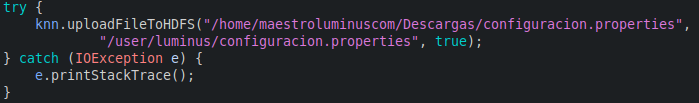
\includegraphics[width=.6\textwidth]{capitulo4b/images/uploadFileToHDFS.png}
		\caption{Subir un archivo previamente creado al HDFS}
		\label{fig:defiQ}
	\end{center}
\end{figure}
En el caso de que se desee crear un archivo o directorio dentro del HDFS sin que este tenga contenido unicamente buscando que este exista y sin la necesidad de crear su equivalente en el equipo local se pueden utilizar las instrucciones mostradas en la figura \ref{fig_defik}. \\ 
\begin{figure}[H]
	\begin{center}
		\hypertarget{fig:defik}{\hspace{1pt}}
		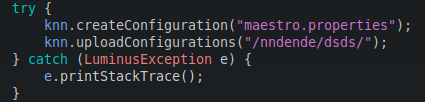
\includegraphics[width=.6\textwidth]{capitulo4b/images/crearysubir.png}
		\caption{Crear archivos en blanco dentro del HDFS}
		\label{fig:defik}
	\end{center}
\end{figure}
Algo importante a tomar en cuenta al momento de realizar estas tareas es que puede que en ocasiones el archivo que se pretende crear o subir al HDFS ya existiera con anterioridad. \\
Haciendo uso de esta función, es posible conocer si el archivo o directorio por el que se pregunta ya se encuentra en el HDFS, en caso de existir se devuelve el valor de True y en caso contrario se devuelve el valor False.
\begin{figure}[H]
	\begin{center}
		\hypertarget{fig:def5}{\hspace{1pt}}
		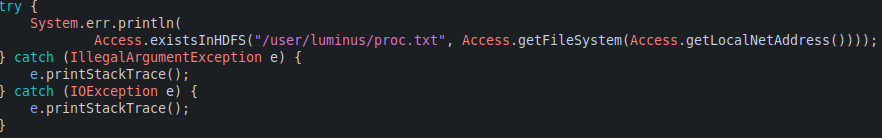
\includegraphics[width=.8\textwidth]{capitulo4b/images/exists.png}
		\caption{Validar si un archivo o directorio existe dentro del HDFS}
		\label{fig:def5}
	\end{center}
\end{figure}
Al finalizar la ejecución de un determinado algoritmo es probable que se requiera obtener una copia del archivo de salidas de manera local, por lo que en este caso se puede utilizar el método que se muestra en la figura \ref{fig:def6}.
\\
Haciendo uso de este método se permite obtener la información contenida dentro del archivo seleccionado.
\begin{figure}[H]
	\begin{center}
		\hypertarget{fig:def6}{\hspace{1pt}}
		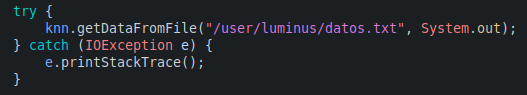
\includegraphics[width=.8\textwidth]{capitulo4b/images/getDataFromFile.png}
		\caption{Validar si un archivo o directorio existe dentro del HDFS}
		\label{fig:def6}
	\end{center}
\end{figure}
\subsubsection{Algoritmo KNN}
Lo primero que se tiene que realizar es la construcción de los elementos que se pasarán a la API como configuraciones para que esta los utilice en su manejo. \\
El número de elementos diferentes que se necesiten de entrada serán definidos propiamente por cada algoritmo que se quiera ejecutar, para los algoritmos establecidos hasta ahora se pueden revisar sus especificaciones en la sección \nameref{disalg} del prototipo \nameref{cap:Cap4.1}\\
En el caso particular del ejemplo se trata de la ejecución del algoritmo KNN, por lo que los datos establecidos en el código fuente del usuario corresponden directamente con este algoritmo. \\
Cabe señalar que estos datos pueden ser construidos de diferentes maneras por el usuario experto y la forma en la que estos se obtengan no tiene injerencia directa con la API.\\
Lo que resulta importante es que una vez que se tenga la totalidad de estos, se tienen que cargar a el método Luminus Configuration KNN.
\begin{figure}[H]
	\begin{center}
		\hypertarget{fig:defi}{\hspace{1pt}}
		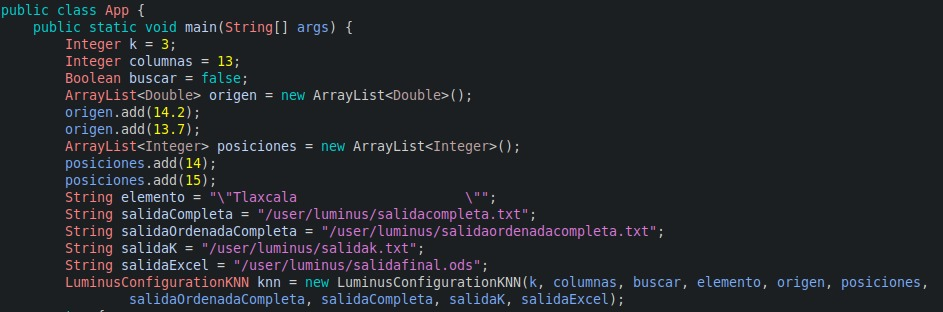
\includegraphics[width=1\textwidth]{capitulo4b/images/uno.jpeg}
		\caption{Definición de elementos necesarios para el funcionamiento del algoritmo KNN}
		\label{fig:defi}
	\end{center}
\end{figure}
Conociendo entonces, los datos de entrada que requieren modificación para la ejecución de este algoritmo en particular que se muestra en la figura \ref{fig:defi}, y ademas de la información de manejo de archivos descrita en la sección \nameref{manarch}, se puede entender con ello la construcción que se realiza en la figura \ref{fig:defichida}. \\
Se presentan 2 nuevas Invocaciones de clases de la API la primera de ellas será útil para revisar si efectivamente el archivo de datos del caso de estudio puede operar con el algoritmo KNN de acuerdo a las columnas seleccionada, en caso de que este no pueda realizarlo regresara un valor false que no permitirá continuar con la ejecución.
La segunda y ultima invocación a clase de la API que se presenta en esta sección permite visualizar una operación de tipo run, esta permite que, una vez que se tienen todas las configuraciones pertenecientes a los algoritmos y ya este listo para ponerse en marcha, esta inicie. \\
Con ello, al finalizar su ejecución se puede tener en el HDFS los resultados de la ejecución.\\
Estas configuraciones representan todo lo necesario para que un algoritmo de KNN pueda iniciar su operación.\\
\begin{figure}[H]
	\begin{center}
		\hypertarget{fig:defichida}{\hspace{1pt}}
		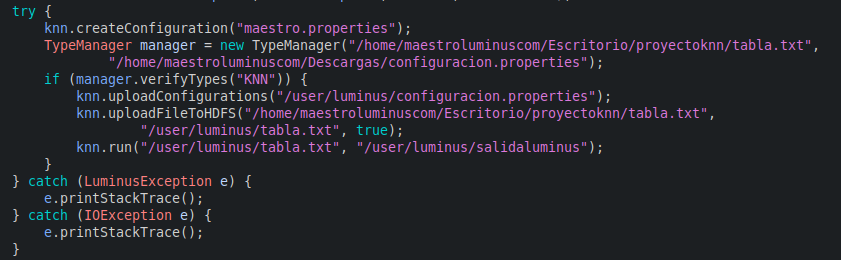
\includegraphics[width=1\textwidth]{capitulo4b/images/apiknn.png}
		\caption{Ejecución knn}
		\label{fig:defichida}
	\end{center}
\end{figure}
\subsubsection{Algoritmo ID3}
De una forma muy similar a como ocurre con el algoritmo KNN este algoritmo, tiene que elaborar sus propias configuraciones de entrada, ya que en caso de no realizarlo, El algoritmo de minería de datos a ejecutar no tendría la información suficiente para comenzar su proceso.\\
De esta manera, nuevamente conociendo cuales son las configuraciones para que este algoritmo opere, unicamente es necesario obtener los datos solicitados por parte del usuario experto.\\
Esta información puede ser obtenida de acuerdo a los medios que el programador de la herramienta que haga uso de Luminus, considere, sin embargo en la figura \ref{fig:dedichida} se puede visualizar la forma en la que esta lo realiza para un determinado caso de uso que puede funcionar con el algoritmo ID3.
\\
Es importante que una vez que se tengan todos los parámetros de configuración distintos estos se manden a la clase LuminusConfigurationID3 para que este tenga conocimiento de esta información para poder comenzar a preparar la ejecución del algoritmo con los datos ingresados.\\
\begin{figure}[H]
	\begin{center}
		\hypertarget{fig:defichida}{\hspace{1pt}}
		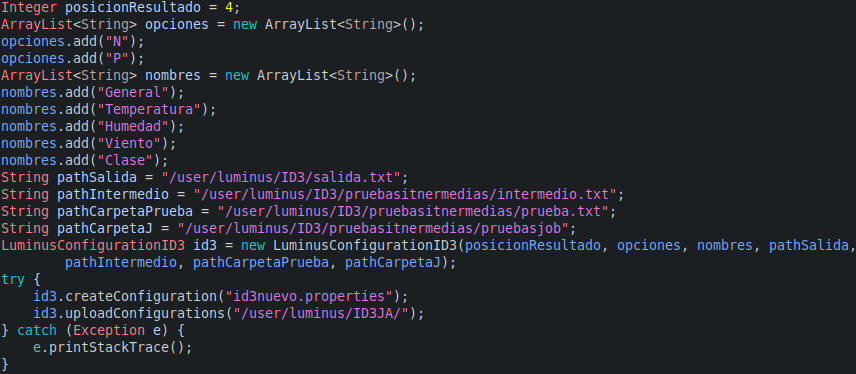
\includegraphics[width=1\textwidth]{capitulo4b/images/id3setup.png}
		\caption{Definición de elementos necesarios para el funcionamiento del algoritmo ID3}
		\label{fig:defichida}
	\end{center}
\end{figure}
De una forma muy similar a la forma de funcionamiento del algoritmo KNN, una vez que se tiene la totalidad de configuraciones realizadas. \\
Es necesario realizar el manejo de archivos correspondiente con respecto al HDFS para poder comenzar la ejecución. para revisar mas a detalle como realizar estas operaciones se puede revisar la sección \nameref{manarch}.
una vez que se tenga preparado este ambiente, solo es necesario iniciar la ejecución del algoritmo lo cual se realiza haciendo uso del método ID3.run.\\
Al finalizar la ejecución de este se tendrán los archivos de salida correctamente escritos con la información relacionada al algoritmo.\\
Finalmente, se pueden eliminar los archivos que se crean para los resultados intermedios en caso de que el usuario experto no tenga interés en ellos, mientras que, si desea conocer los resultados obtenidos a cada iteración puede ser información de utilidad para este usuario. Por esta razón se deja a criterio del usuario si desea realizar su eliminación y en que momento desea hacerlo.
\begin{figure}[H]
	\begin{center}
		\hypertarget{fig:defichida1}{\hspace{1pt}}
		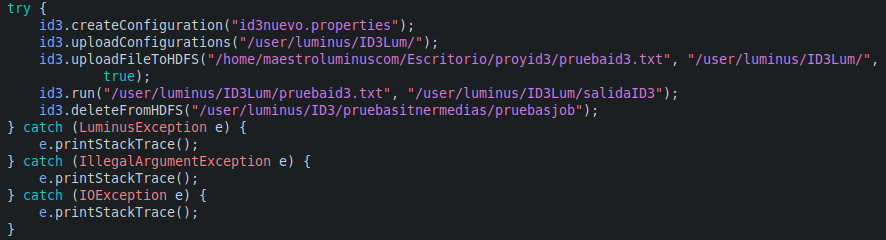
\includegraphics[width=1\textwidth]{capitulo4b/images/ID3exec.png}
		\caption{Ejecución ID3}
		\label{fig:defichida1}
	\end{center}
\end{figure}